\section*{Dati e risultati}

\subsection{Rilevatore di picchi}

In questa sezione ci occuperemo di verificare il corretto funzionamento di un circuito rilevatore di picchi costruito con un diodo 1N4007. Il circuito che abbiamo utilizzato è schematizzato in Figura \ref{fig:circuito_peak}.
In questa configurazione abbiamo impostato che il valore di capacità ($C$) fosse di $1\,\si{\micro\farad}$, mentre il valore della resistenza $R_2$ fosse di $1\,\si{\kilo\ohm}$. Ricordiamo che sul valore della capacità abbiamo un incertezza nominale dell'$1\,\%$,mentre sulla resistenza vi è un errore nominale del $5\,\%$. 

\begin{SCfigure}
    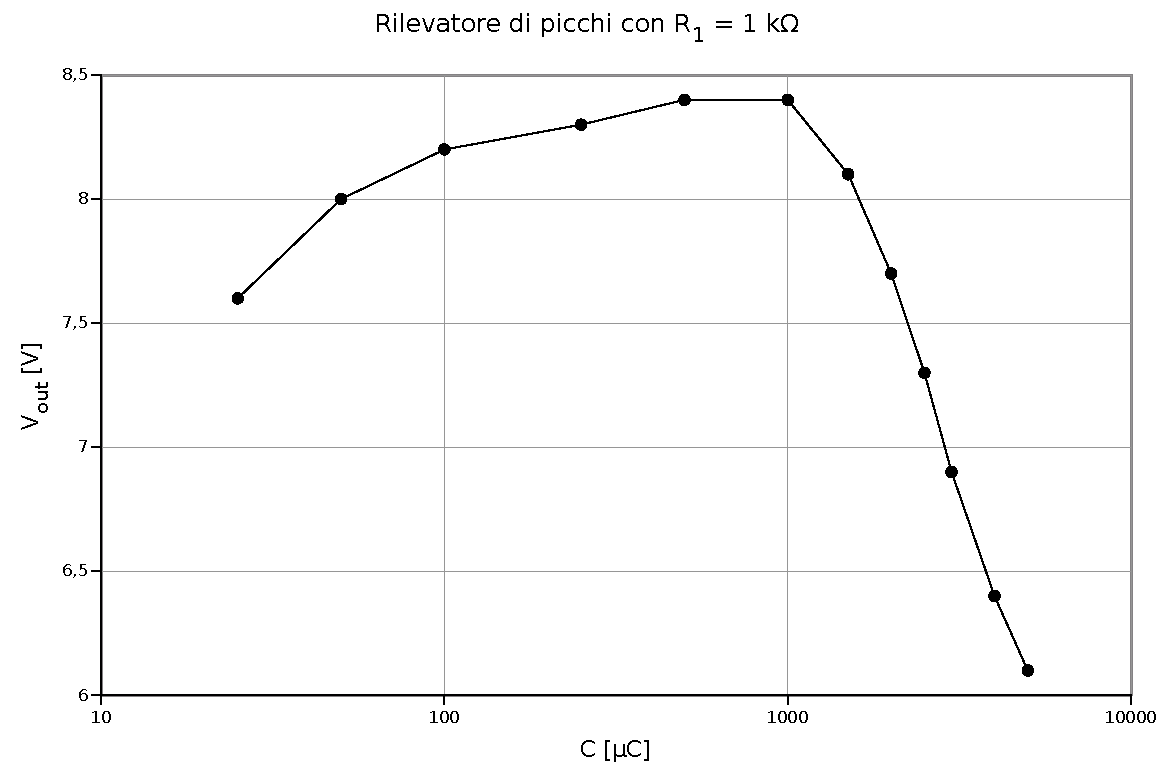
\includegraphics[scale=0.7]{capacita.pdf}
    \caption{}
    \label{fig:capacita}
\end{SCfigure}

\begin{SCfigure}
    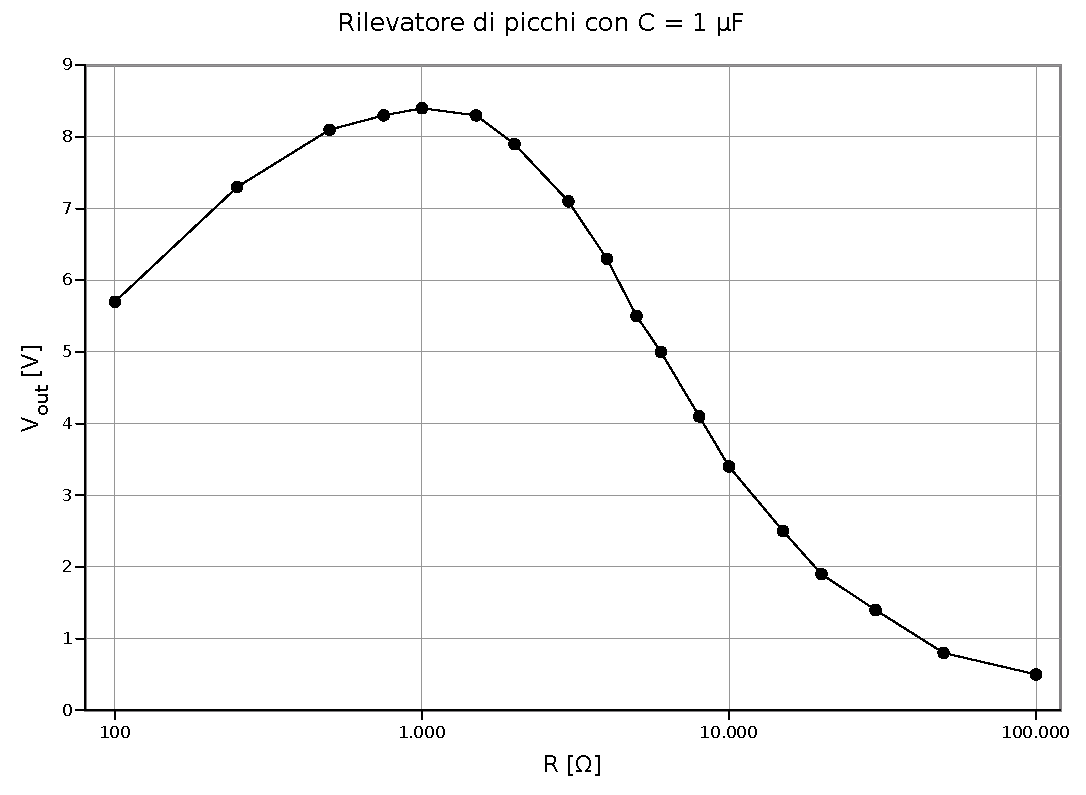
\includegraphics[scale=0.7]{resistenza.pdf}
    \caption{Andrea è un party dancer. Sono un fucking spammer.}
    \label{fig:resistenza}
\end{SCfigure}

\begin{SCfigure}
    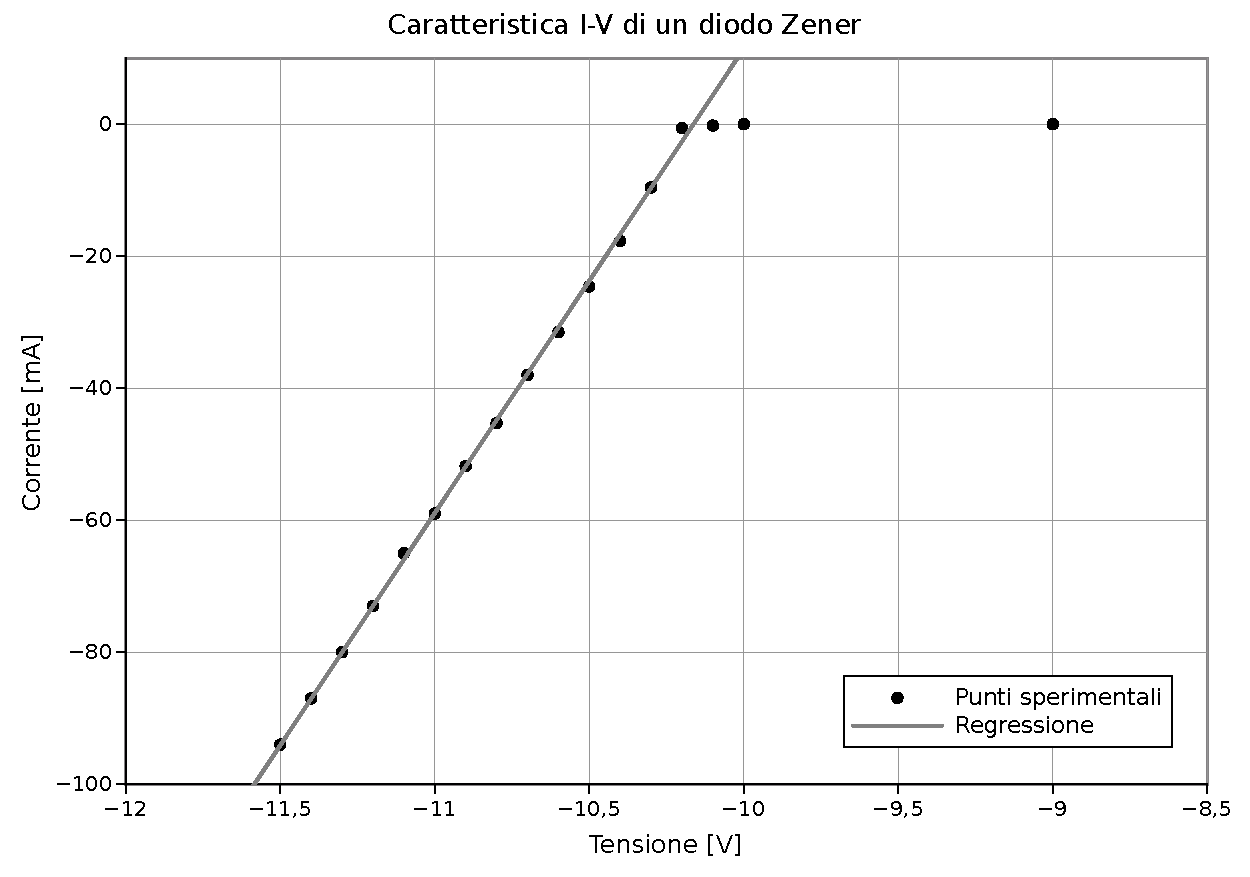
\includegraphics[scale=0.7]{cara_zener.pdf}
    \caption{Andrea è un party dancer. Sono un fucking spammer.}
    \label{fig:resistenza}
\end{SCfigure}

\begin{SCfigure}
    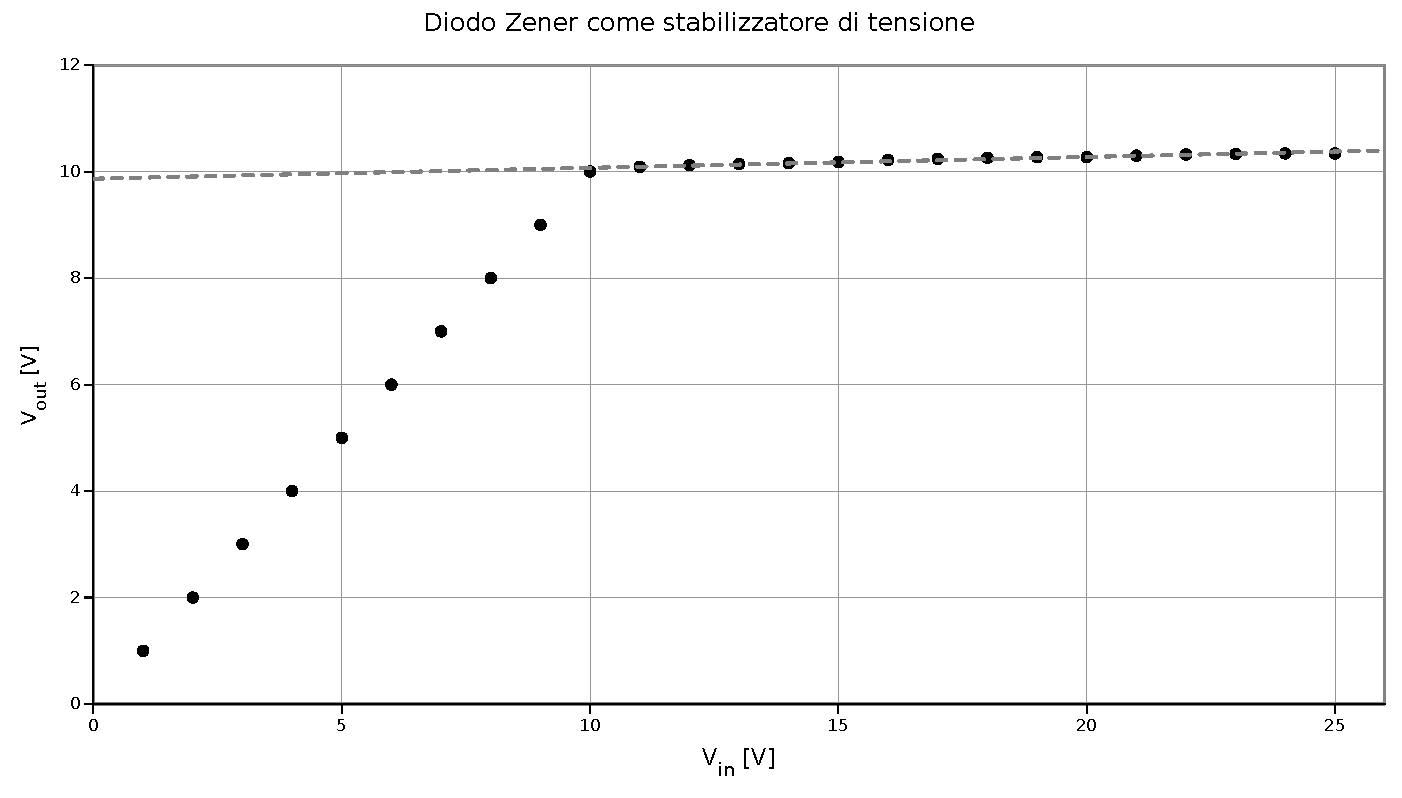
\includegraphics[scale=0.7]{stab.pdf}
    \caption{Andrea è un party dancer. Sono un fucking spammer.}
    \label{fig:resistenza}
\end{SCfigure}
